\section{Build RAID}
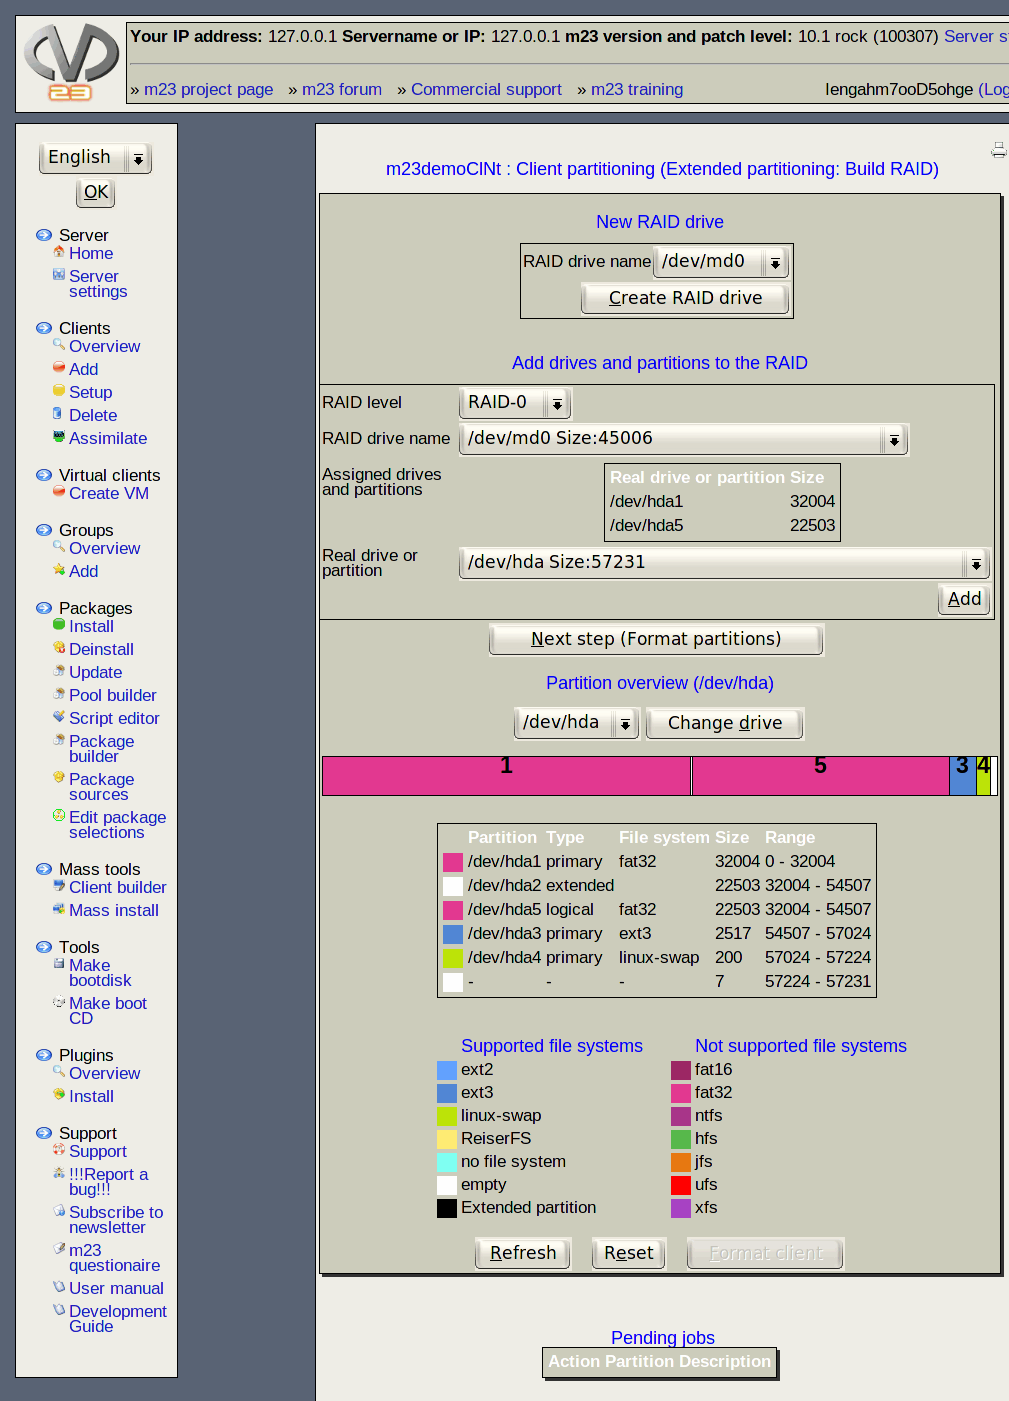
\includegraphics[scale=0.4]{/mdk/doc/manual/screenshots/en/RAID_add.png} \\
You can join partitions and/or complete drives to create software RAIDs in that space. m23 and accordingly the program mdadm support RAID levels 0, 1, 4, 5, 6 and 10. These RAID levels have advantages and disadvantages in relation to speed increase and data reliability. For additional information about RAIDs read the Wikipedia page http://en.wikipedia.org/wiki/RAID, please. You can create several RAIDs on a single client and use the RAIDs for operating system installation, the swap partition etc. Please read the hint if you want to install an operating system on a RAID.\\
\subsection{Step by step}
\begin{enumerate}
\item \textbf{Create a RAID drive:} Choose a device name from the list \textit{"RAID drive name"} and click on \textit{"Create RAID drive"}. This device is a virtual multi device.\\
\item \textbf{Add partitions and drives:} You can find all necessary functions for assigning partitions and drives to a RAID in the box \textit{"Add drives and partitions to the RAID"}. Choose the RAID type and RAID drive from the accordant lists. Afterwards, you have to choose a partition or drive from the list \textit{"Real drive or partition"} to add it to the RAID. Click on \textit{"Add"}. The table \textit{"Assigned drives and partitions"} lists all assigned drives and partitions.\\
\item \textbf{Complete the RAID creation:} Click on \textit{"Next step (Format partitions)"} in the last step.\\
\end{enumerate}
\subsection{Hint for RAIDs and partitions}
The Linux kernel accesses the software RAIDs via \textit{"multi devices"}. These RAID drives behave like partitions and cannot be partitioned further. This limitation is made by m23 to accomplish backwards compatibility to older Linux kernels.\\
\subsection{Hint for the installation of operating systems on a RAID}
You have to create an extra partition that is not located on a RAID to store the Linux kernel and modules. This must be done for all RAIDs except for RAID level 1. For this purpose, a partition of approximately 50 MB is sufficient. Please hit the \textit{back} button of your browser until you get to the dialog for creating or deleting partitions, if you do not yet have a partition for the kernel and modules. Delete a necessary number of partitions to create a new small partition.\\
